\chapter{Appendix for Chapter \ref{chp3}} \label{app:c}

\section{Conditional Survival Probability}

\begin{flalign}
 S_{li}(t'|t) & = p(t_{n_{li}+1} \geq t'|t_{n_{li}+1} > t,\mathcal{D})&&\\\nonumber
              & = \int\int\int\int p(t_{n_{li}+1} \geq t'|t_{n_{li}+1} > t, b_l,\bm{U}_{li},v_{li},\bm{\theta},\mathcal{D}) \cdot p(b_l, \bm{U}_{li}, v_{li}, \bm{\theta} |t_{n_{li}+1} > t, \mathcal{D}) \, db_l \, d\bm{U}_{li} \, dv_{li} \, d\bm{\theta}&& \nonumber \\
              & = \int\int\int\int \frac{p(t_{n_{li}+1} \geq t'|b_l, \bm{U}_{li}, v_{li}, \bm{\theta})}{p(t_{n_{li}+1} > t|b_l, \bm{U}_{li}, v_{li}, \bm{\theta})} \cdot p(b_l, \bm{U}_{li}, v_{li}, \bm{\theta} |t_{n_{li}+1} > t, \mathcal{D}) \, db_l \, d\bm{U}_{li} \, dv_{li} \, d\bm{\theta}&& \nonumber \\
              & = \int\int\int\int \frac{S(t'|b_l, \bm{U}_{li}, v_{li}, \bm{\theta})}{S(t|b_l, \bm{U}_{li}, v_{li}, \bm{\theta})} \cdot p(b_l, \bm{U}_{li}, v_{li}, \bm{\theta} |t_{n_{li}+1} > t, \mathcal{D}) \, db_l \, d\bm{U}_{li} \, dv_{li} \, d\bm{\theta}&& \nonumber \\
              &=\int\int\int\int \frac{exp\Big[-\int_{0}^{t'}h(s|b_l, \bm{U}_{li}, v_{li}, \bm{\theta})ds\Big]}{exp\Big[-\int_{0}^{t}h(s|b_l, \bm{U}_{li}, v_{li}, \bm{\theta})ds\Big]} \cdot p(b_l, \bm{U}_{li}, v_{li}, \bm{\theta} |t_{n_{li}+1} > t, \mathcal{D}) \, db_l \, d\bm{U}_{li} \, dv_{li} \, d\bm{\theta}&& \nonumber \\
              &=\int\int\int\int exp\Big[-\int_{t}^{t'}h(s|b_l, \bm{U}_{li}, v_{li}, \bm{\theta})ds\Big] \cdot p(b_l, \bm{U}_{li}, v_{li}, \bm{\theta} |t_{n_{li}+1} > t, \mathcal{D}) \, db_l \, d\bm{U}_{li} \, dv_{li} \, d\bm{\theta}&& \nonumber \\
              & \approx \frac{1}{M} \sum_{m=1}^{M} exp\Big[ -\int_t^{t'} h\big(s|b_l^{(m)},\bm{U}_{li}^{(m)},v_{li}^{(m)},\bm{\theta}^{(m)}\big) ds \Big] \nonumber
\end{flalign}

\section{Simulation Results}

\begin{center}
\begin{table}[H]
\caption{Simulation results under models with current slope as association structure across gap \& calendar risk intervals}
 \centering
 \begin{threeparttable}
  \begin{tabular}{lrllrllrllrll}
    \toprule
   & \multicolumn{6}{c} {SLOPE+GAP} & \multicolumn{6}{c} {SLOPE+CAL}\\
    \cmidrule(lr) {2-7} 
    \cmidrule(lr) {8-13} 
  Parameter & \multicolumn{3}{c}{Joint Model} & \multicolumn{3}{c}{Two-stage Model} & \multicolumn{3}{c}{Joint Model} & \multicolumn{3}{c}{Two-stage Model}  \\
 \cmidrule(lr) {2-4}  \cmidrule(lr) {5-7}
 \cmidrule(lr) {8-10}  \cmidrule(lr) {11-13}
 & Bias \tnote{a} & SE \tnote{b} & C90 \tnote{c} & Bias \tnote{a} & SE \tnote{b} & C90 \tnote{c} & Bias \tnote{a} & SE \tnote{b} & C90 \tnote{c} & Bias \tnote{a} & SE \tnote{b} & C90 \tnote{c} \\
 \midrule 
 \rowcolor{Gainsboro!60}
 \multicolumn{13}{l}{\bf Longitudinal submodel}\\
  $\beta_0$ & -0.20 & 0.36 & 0.86 & -0.24 & 0.37 & 0.86 & 0.23 & 0.32 & 0.92 & 0.18 & 0.32 & 0.92\\
  $\beta_1$ & 0.02 & 0.05 & 0.94 & -0.11 & 0.06 & 0.92 & 0.09 & 0.06 & 0.88 & 0.10 & 0.07 & 0.84\\
  $\beta_2$ & -0.01 & 0.01 & 0.94 & 0.01 & 0.01 & 0.90 & -0.01 & 0.01 & 0.88 & 0.00 & 0.01 & 0.88\\
  $\sigma$ & -0.19 & 0.06 & 0.90 & -0.18 & 0.06 & 0.90 & -0.07 & 0.06 & 0.90 & -0.03 & 0.06 & 0.90\\
  $\sigma_b$ & -0.42 & 0.25 & 0.98 & -0.39 & 0.24 & 0.98 & -0.20 & 0.28 & 0.98 & -0.21 & 0.28 & 0.96\\
  $\sigma_{u0}$ & 0.06 & 0.11 & 0.94 & 0.09 & 0.11 & 0.94 & -0.12 & 0.11 & 0.92 & -0.14 & 0.12 & 0.92\\
  $\sigma_{u1}$ & 0.04 & 0.02 & 0.92 & 0.03 & 0.02 & 0.90 & 0.01 & 0.02 & 0.96 & -0.01 & 0.02 & 0.96\\
  $\rho$ & -0.01 & 0.01 & 0.90 & -0.01 & 0.01 & 0.94 & 0.00 & 0.01 & 0.84 & 0.01 & 0.01 & 0.86\\
  \rowcolor{Gainsboro!60}
  \multicolumn{13}{l}{\bf Event submodel}\\
  $\gamma_0$ & 0.38 & 0.07 & 0.70 & 0.32 & 0.06 & 0.68 & 0.22 & 0.04 & 0.82 & 0.20 & 0.04 & 0.80\\
  $\gamma_1$ & 0.01 & 0.04 & 0.88 & 0.00 & 0.04 & 0.88 & -0.03 & 0.03 & 0.96 & -0.03 & 0.03 & 0.96\\
  $\gamma_2$ & 0.03 & 0.02 & 0.90 & 0.03 & 0.02 & 0.90 & 0.03 & 0.02 & 0.90 & 0.03 & 0.02 & 0.90\\
  $\delta_1$ & -0.08 & 0.02 & 0.84 & -0.07 & 0.02 & 0.84 & -0.03 & 0.02 & 0.86 & -0.02 & 0.02 & 0.88\\
  $\delta_2$ & -0.05 & 0.02 & 0.90 & -0.04 & 0.02 & 0.90 & -0.01 & 0.02 & 0.90 & -0.01 & 0.02 & 0.78\\
  $\delta_3$ & -0.10 & 0.03 & 0.80 & -0.07 & 0.03 & 0.82 & -0.02 & 0.02 & 0.94 & -0.02 & 0.02 & 0.94\\
  $\delta_4$ & -0.08 & 0.03 & 0.84 & -0.05 & 0.03 & 0.84 & 0.01 & 0.02 & 0.94 & 0.01 & 0.02 & 0.94\\
  $\delta_5$ & -0.06 & 0.02 & 0.88 & -0.05 & 0.02 & 0.90 & 0.00 & 0.03 & 0.90 & 0.01 & 0.03 & 0.88\\
  $\delta_6$ & -0.07 & 0.02 & 0.88 & -0.05 & 0.02 & 0.88 & -0.04 & 0.03 & 0.88 & -0.04 & 0.02& 0.90\\
  $\alpha_1$ & 0.02 & 0.01 & 0.88 & 0.01 & 0.01 & 0.84 & 0.01 & 0.01 & 0.98 & 0.01 & 0.01 & 0.94\\
  $\alpha_2$ & 0.01 & 0.01 & 0.88 & 0.00 & 0.01 & 0.88 & 0.02 & 0.01 & 0.94 & 0.02 & 0.01 & 0.92\\
  $\alpha_3$ & -0.02 & 0.02 & 0.86 & -0.01 & 0.02 & 0.86 & 0.02 & 0.02 & 0.86 & 0.02 & 0.02 & 0.86\\
  $\alpha_4$ & -0.05 & 0.02 & 0.86 & -0.04 & 0.02 & 0.84 & 0.00 & 0.02 & 0.94 & 0.00 & 0.02 & 0.92\\
  $\alpha_5$ & -0.03 & 0.02 & 0.86 & -0.03 & 0.02 & 0.88 & 0.01 & 0.01 & 0.94 & 0.01 & 0.01 & 0.96\\
  $\alpha_6$ & -0.01 & 0.02 & 0.86 & -0.01 & 0.02 & 0.90 & -0.01 & 0.01 & 0.92 & -0.01 & 0.01 & 0.92\\
  $\sigma_v$ & -0.14 & 0.02 & 0.76 & -0.15 & 0.02 & 0.78 & -0.08 & 0.02 & 0.90 & -0.10 & 0.02 & 0.92\\
    \bottomrule
  \end{tabular}
   \begin{tablenotes}[para]
    \footnotesize
        \item[a] Bias=true value-mean estimate; \item[b] SE=standard error; \item[c] C90= probability of 90\% coverage 
    \end{tablenotes}
    \end{threeparttable}
\end {table}
\end{center}

\begin{center}
\begin{table}[H]
\caption{Simulation results under models with current value as association structure across gap \& calendar risk intervals}
 \centering
 \begin{threeparttable}
  \begin{tabular}{lrllrllrllrll}
    \toprule
   & \multicolumn{6}{c} {VALUE+GAP} & \multicolumn{6}{c} {VALUE+CAL}\\
    \cmidrule(lr) {2-7} 
    \cmidrule(lr) {8-13} 
  Parameter & \multicolumn{3}{c}{Joint Model} & \multicolumn{3}{c}{Two-stage Model} & \multicolumn{3}{c}{Joint Model} & \multicolumn{3}{c}{Two-stage Model}  \\
 \cmidrule(lr) {2-4}  \cmidrule(lr) {5-7}
 \cmidrule(lr) {8-10}  \cmidrule(lr) {11-13}
 & Bias \tnote{a} & SE \tnote{b} & C90 \tnote{c} & Bias \tnote{a} & SE \tnote{b} & C90 \tnote{c} & Bias \tnote{a} & SE \tnote{b} & C90 \tnote{c} & Bias \tnote{a} & SE \tnote{b} & C90 \tnote{c} \\
 \midrule 
 \rowcolor{Gainsboro!60}
 \multicolumn{13}{l}{\bf Longitudinal submodel}\\
  $\beta_0$ & 0.07 & 0.33 & 0.90 & 0.08 & 0.33 & 0.92 & -0.34 & 0.32 & 0.96 & -0.30 & 0.32 & 0.96\\
  $\beta_1$ & 0.05 & 0.06 & 0.96 & 0.20 & 0.06 & 0.90 & 0.00 & 0.05 & 0.92 & 0.11 & 0.06 & 0.92 \\
  $\beta_2$ & 0.00 & 0.01 & 0.86 & -0.02 & 0.01 & 0.84 & 0.00 & 0.01 & 0.94 & -0.02 & 0.01 & 0.90 \\
  $\sigma$ & -0.07 & 0.05 & 0.90 & -0.06 & 0.05 & 0.90 & 0.00 & 0.05 & 0.90 & 0.02 & 0.05 & 0.92 \\
  $\sigma_b$ & -0.12 & 0.30 & 0.96 & -0.18 & 0.28 & 0.96 & -0.94 & 0.28 & 0.90 & -0.89 & 0.28 & 0.92 \\
  $\sigma_{u0}$ & -0.13 & 0.11 & 0.94 & -0.15 & 0.11 & 0.94 & 0.00 &  0.11 & 0.92 & -0.05 & 0.11 & 0.92 \\
  $\sigma_{u1}$ & -0.01 & 0.02 & 0.98 & -0.02 & 0.02 & 0.98 & 0.01 &  0.02 & 0.94 & 0.00 & 0.02 & 0.92 \\
  $\rho$ & -0.01 & 0.01 & 0.94 & -0.01 & 0.01 & 0.94 & 0.01 & 0.01 &  0.94 & 0.01 & 0.01 & 0.96 \\
  \rowcolor{Gainsboro!60}
  \multicolumn{13}{l}{\bf Event submodel}\\
  $\gamma_0$ & 0.21 & 0.05 & 0.86 & 0.18 & 0.05 & 0.86 & 0.31 & 0.06 & 0.86 & 0.27 & 0.06 & 0.88\\
  $\gamma_1$ & -0.06 & 0.05 & 0.90 & -0.06 & 0.05 & 0.90 & -0.02 & 0.04 & 0.98 & -0.02 & 0.04 & 0.98 \\
  $\gamma_2$ & -0.03 & 0.02 & 0.96 & -0.03 & 0.02 & 0.96 & -0.04 & 0.02 & 0.92& -0.04 & 0.02 & 0.92\\
  $\delta_1$ & -0.11 & 0.03 & 0.90 & -0.10 & 0.03 & 0.86 & -0.06 & 0.03 & 0.82 & -0.05 & 0.03 & 0.80\\
  $\delta_2$ & -0.03 & 0.03 & 0.90 & -0.02 & 0.03 & 0.88 & 0.82 & 0.03 & 0.96 & -0.07 & 0.03 & 0.98\\
  $\delta_3$ & -0.07 & 0.02 & 0.90 & -0.06 & 0.02 & 0.92 & -0.04 & 0.03 & 0.92 & -0.04 & 0.03 & 0.92\\
  $\delta_4$ & -0.02 & 0.02 & 0.94 & -0.02 & 0.02 & 0.94 & -0.02 & 0.02 & 0.92 & -0.02 & 0.02 & 0.92\\
  $\delta_5$ & -0.06 & 0.02 & 0.88 & -0.06 & 0.02 & 0.92 & -0.05 & 0.02 & 0.96 & -0.05 & 0.02 & 0.96\\
  $\delta_6$ & -0.02 & 0.03 & 0.92 & -0.01 & 0.03 & 0.90 & -0.06 & 0.03 & 0.88 & -0.05 & 0.03 & 0.86\\
  $\alpha_1$ & 0.00 & 0.00 & 0.88 & 0.00 & 0.00 & 0.86 & 0.00 & 0.00 & 0.88 & 0.00 & 0.00 & 0.88\\
  $\alpha_2$ & 0.00 & 0.00 & 0.90 & 0.00 & 0.00 & 0.88 & 0.00 & 0.00 & 0.92 & 0.00 & 0.00 & 0.92\\
  $\alpha_3$ & 0.00 & 0.00 & 0.84 & 0.00 & 0.00 & 0.82 & 0.00 & 0.00 & 0.88 & 0.00 & 0.00 & 0.88\\
  $\alpha_4$ & 0.00 & 0.00 & 0.92 & 0.00 & 0.00 & 0.92 & 0.00 & 0.00 & 0.96 & 0.00 & 0.00 & 0.96\\
  $\alpha_5$ & 0.00 & 0.00 & 0.86 & 0.00 & 0.00 & 0.86 & 0.00 & 0.00 & 0.88 & 0.00 & 0.00 & 0.88\\
  $\alpha_6$ & 0.00 & 0.00 & 0.86 & 0.00 & 0.00 & 0.88 & 0.00 & 0.00 & 0.88 & 0.00 & 0.00 & 0.90\\
  $\sigma_v$ & -0.16 & 0.03 & 0.80 & -0.16 & 0.03 & 0.78 & -0.05 & 0.03 & 0.88 & -0.05 & 0.03 & 0.90\\
    \bottomrule
  \end{tabular}
   \begin{tablenotes}[para]
    \footnotesize
        \item[a] Bias=true value-mean estimate; \item[b] SE=standard error; \item[c] C90=probability of 90\% credible interval coverage 
    \end{tablenotes}
    \end{threeparttable}
\end {table}
\end{center}

\section{Real Data}

\begin{figure}[H]
\centering
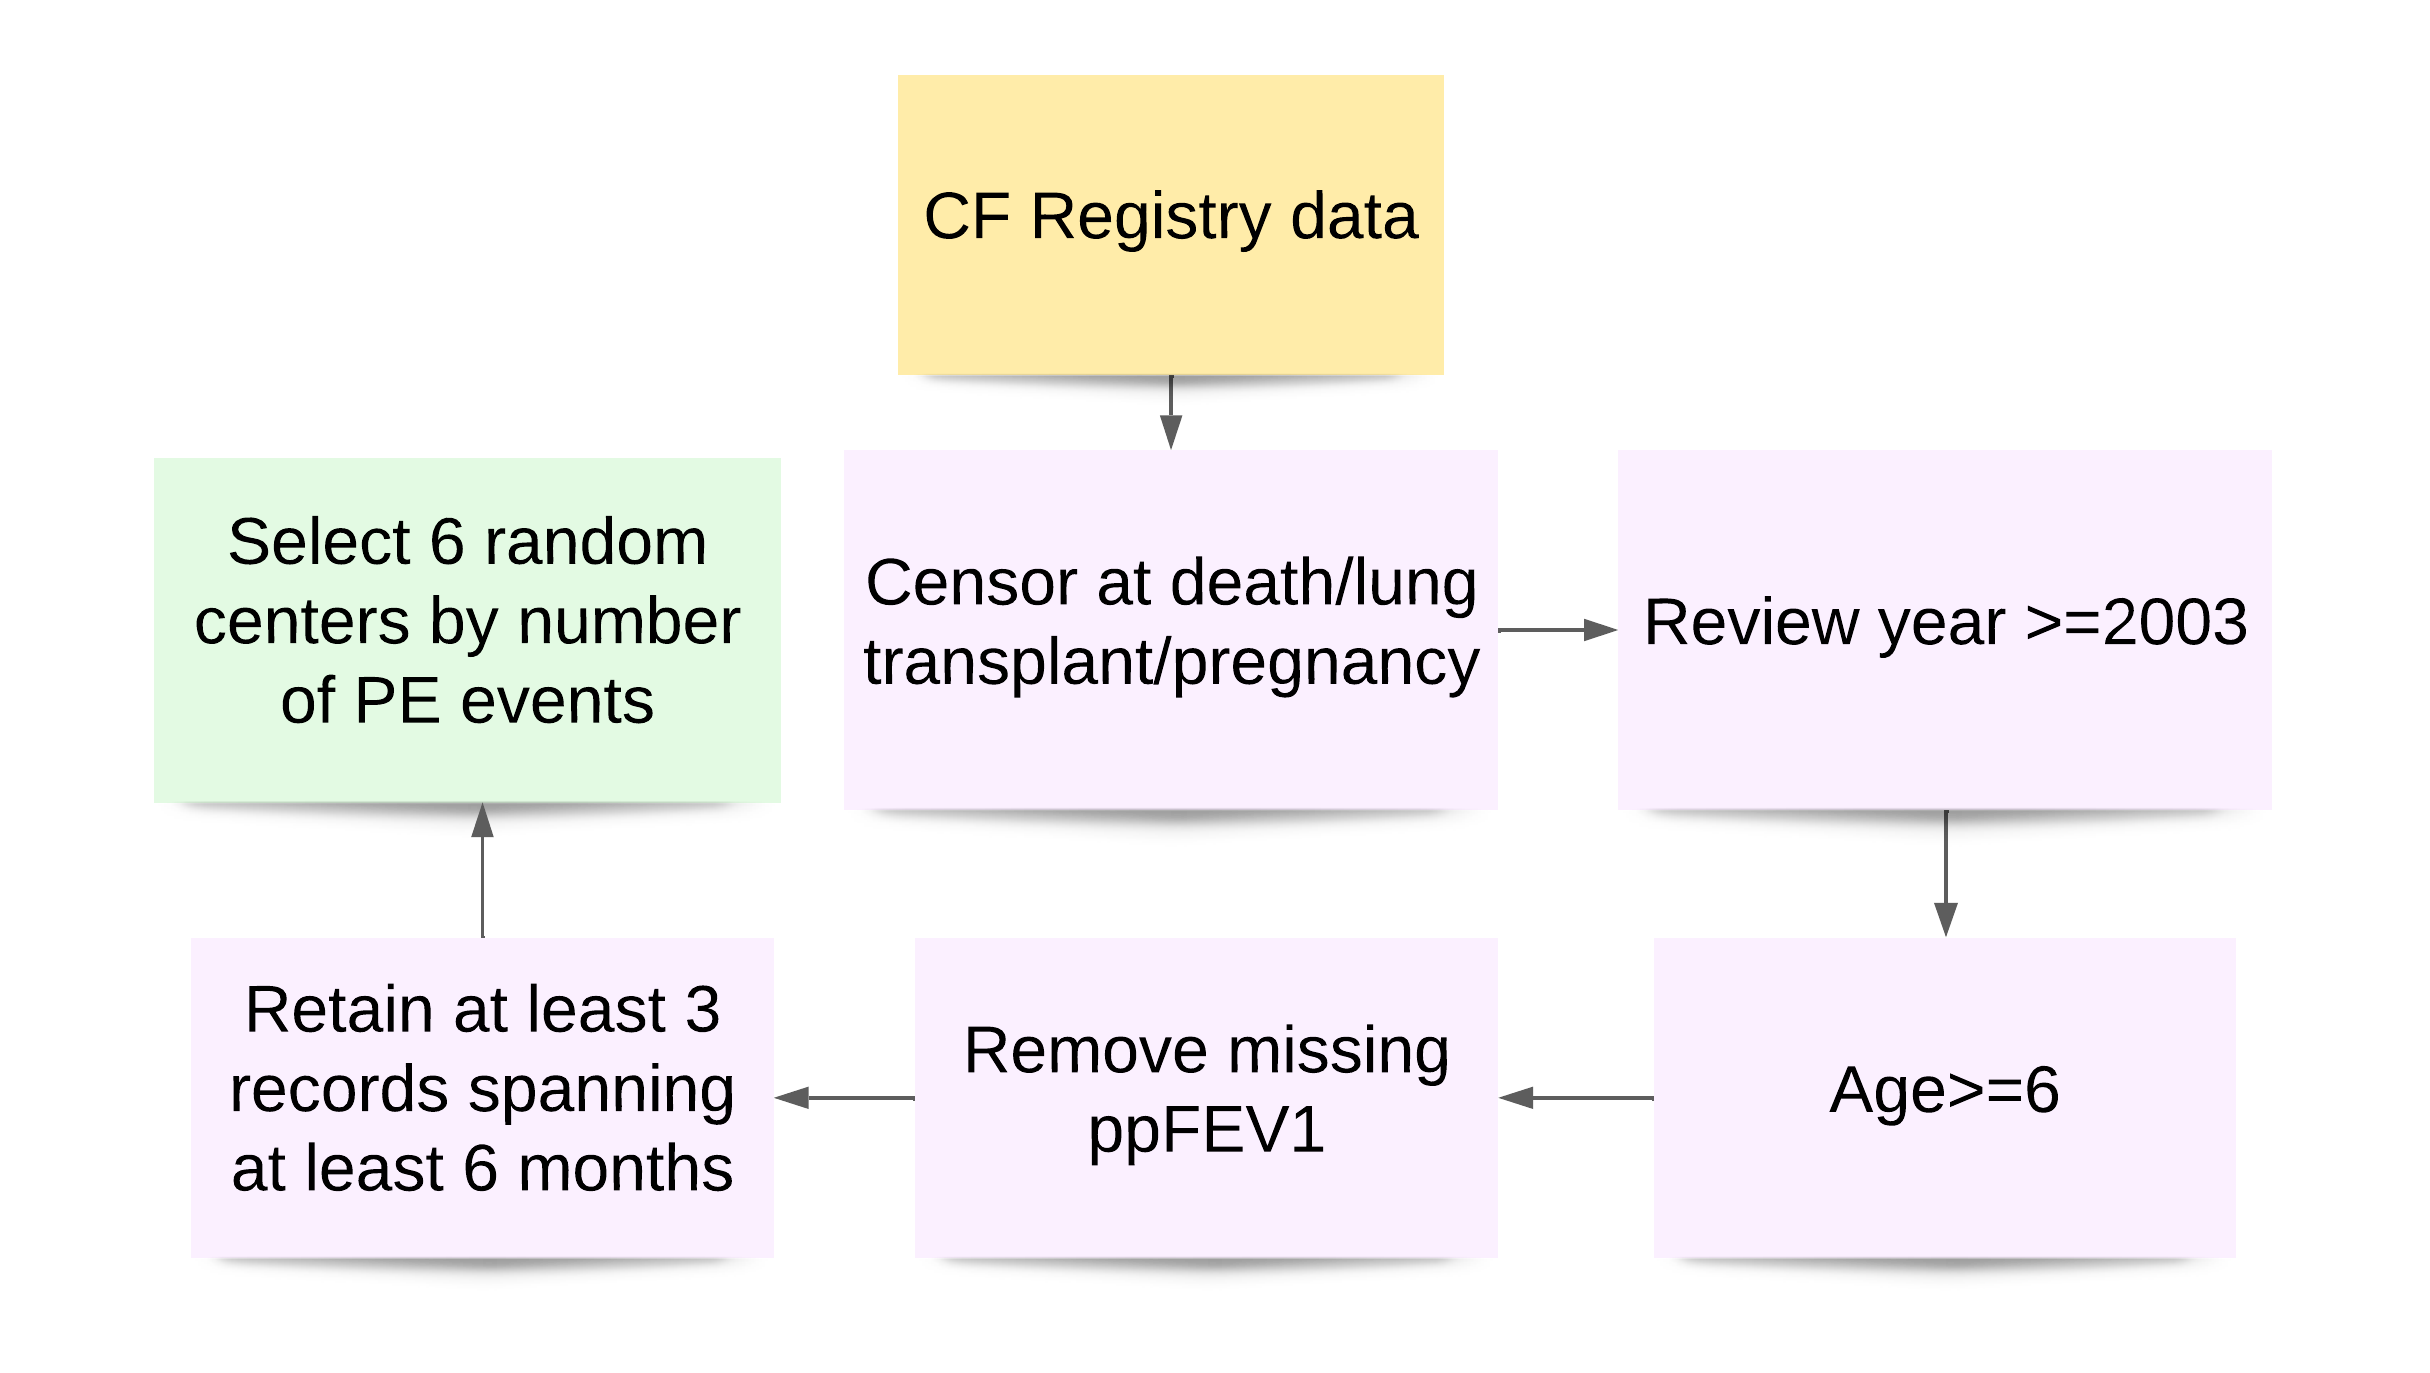
\includegraphics[width=\textwidth]{Figures/Chp3_data_diag.png}
\caption{Data cleaning process}
\end{figure}

\section{Convergence Diagnostics}

In this section, we have investigated some common visual MCMC diagnostics using the R bayesplot (\cite{bayesplot2020}) package for our optimal model. The time series plot of the Markov chains is shown in Figure \ref{fig:trace}. Typically we can see that both chains explore the similar region of parameter values, which is a good sign. We can also visualize the ACF for each Markov chain separately up to a lag of 20 for each parameter. We prefer ACF to drop quickly to zero with increasing lag because positive autocorrelation means the chain tends to stay in the same area between iterations. All parameters are shown to meet this expectation from Figure \ref{fig:acf_long} and Figure \ref{fig:acf_surv}. It is notable that negative autocorrelation is possible and it indicates fast convergence of sample mean towards true mean.  

The motivation of the potential scale reduction statistic($\hat{R}$) is to measure the ratio of the average variance of draws within each chain to the variance of pooled draws across chains. If the chains have not converged to a common distribution, the $\hat{R}$ statistic will be greater than one (\cite{Gelman2013b},\cite{Rstan2020}). The points in Figure \ref{fig:rhat} representing $\hat{R}$ values are colored based on some cutoffs and there are no divergences observed.   

\begin{figure}[H] 
\centering
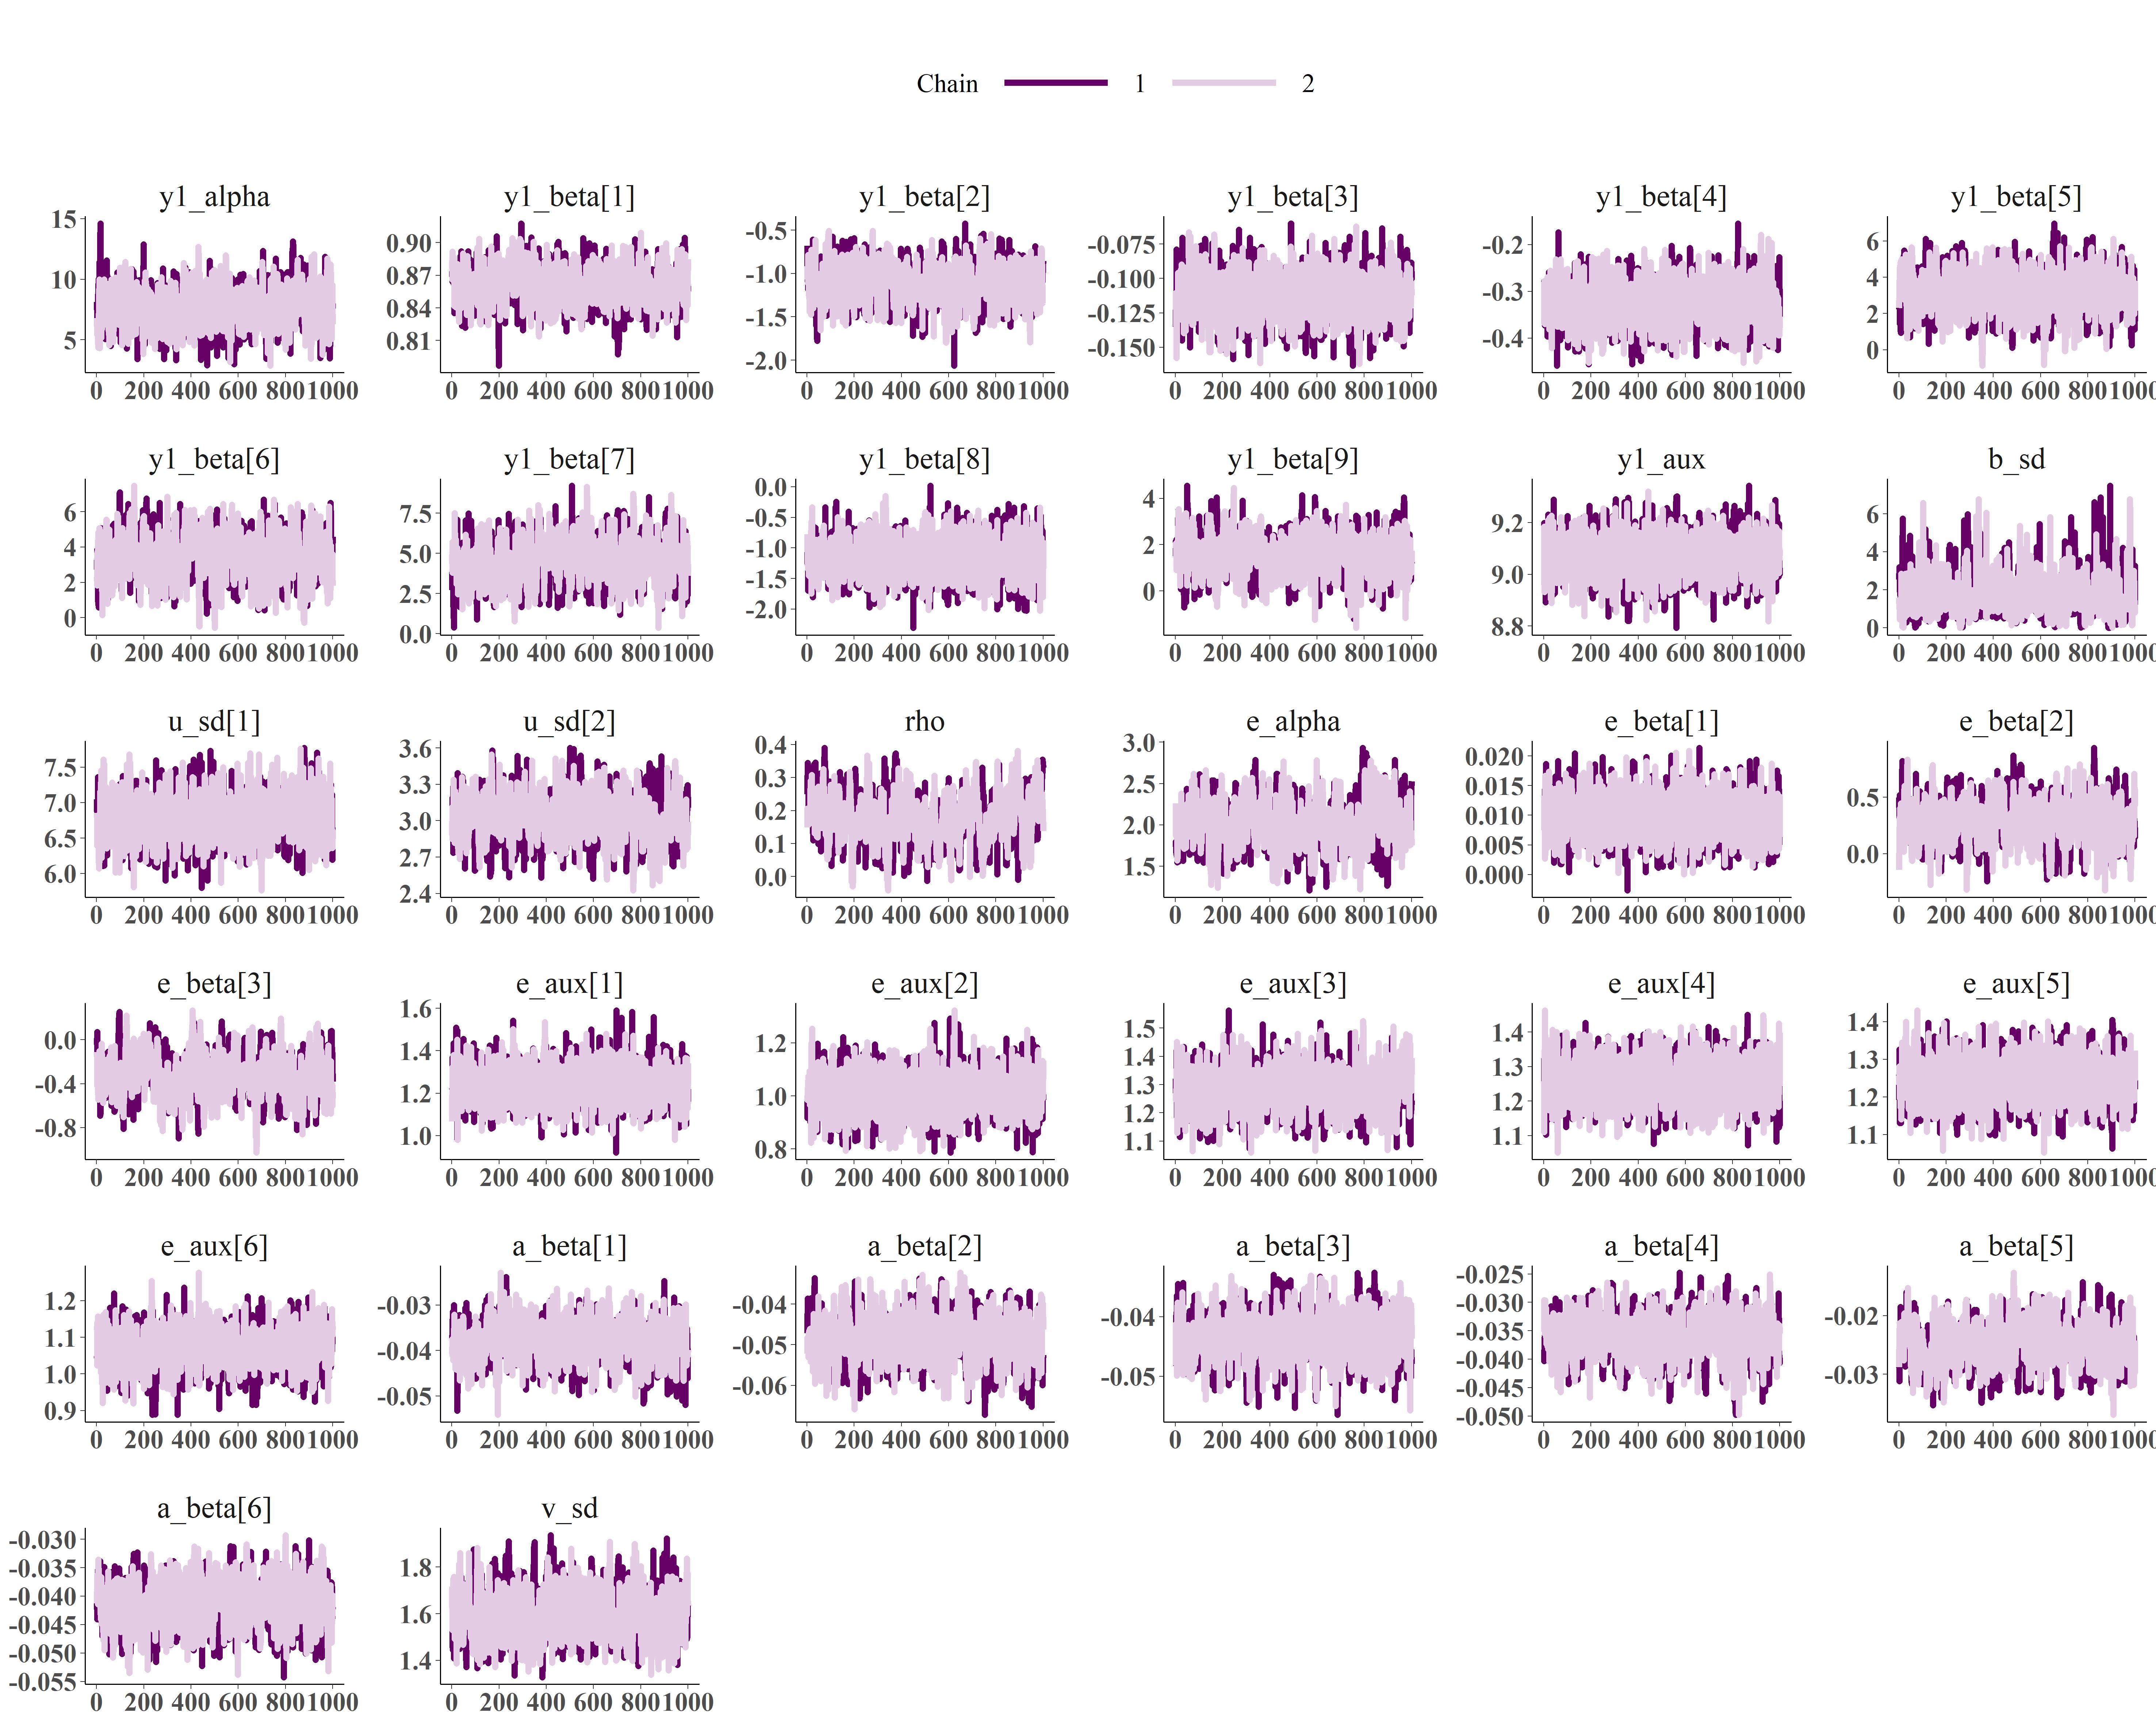
\includegraphics[width=\textwidth]{Figures/Chp3_traceplot.jpg}
\caption{Traceplot against iterations}
\label{fig:trace}
\end{figure}

\begin{figure}[H] 
\centering
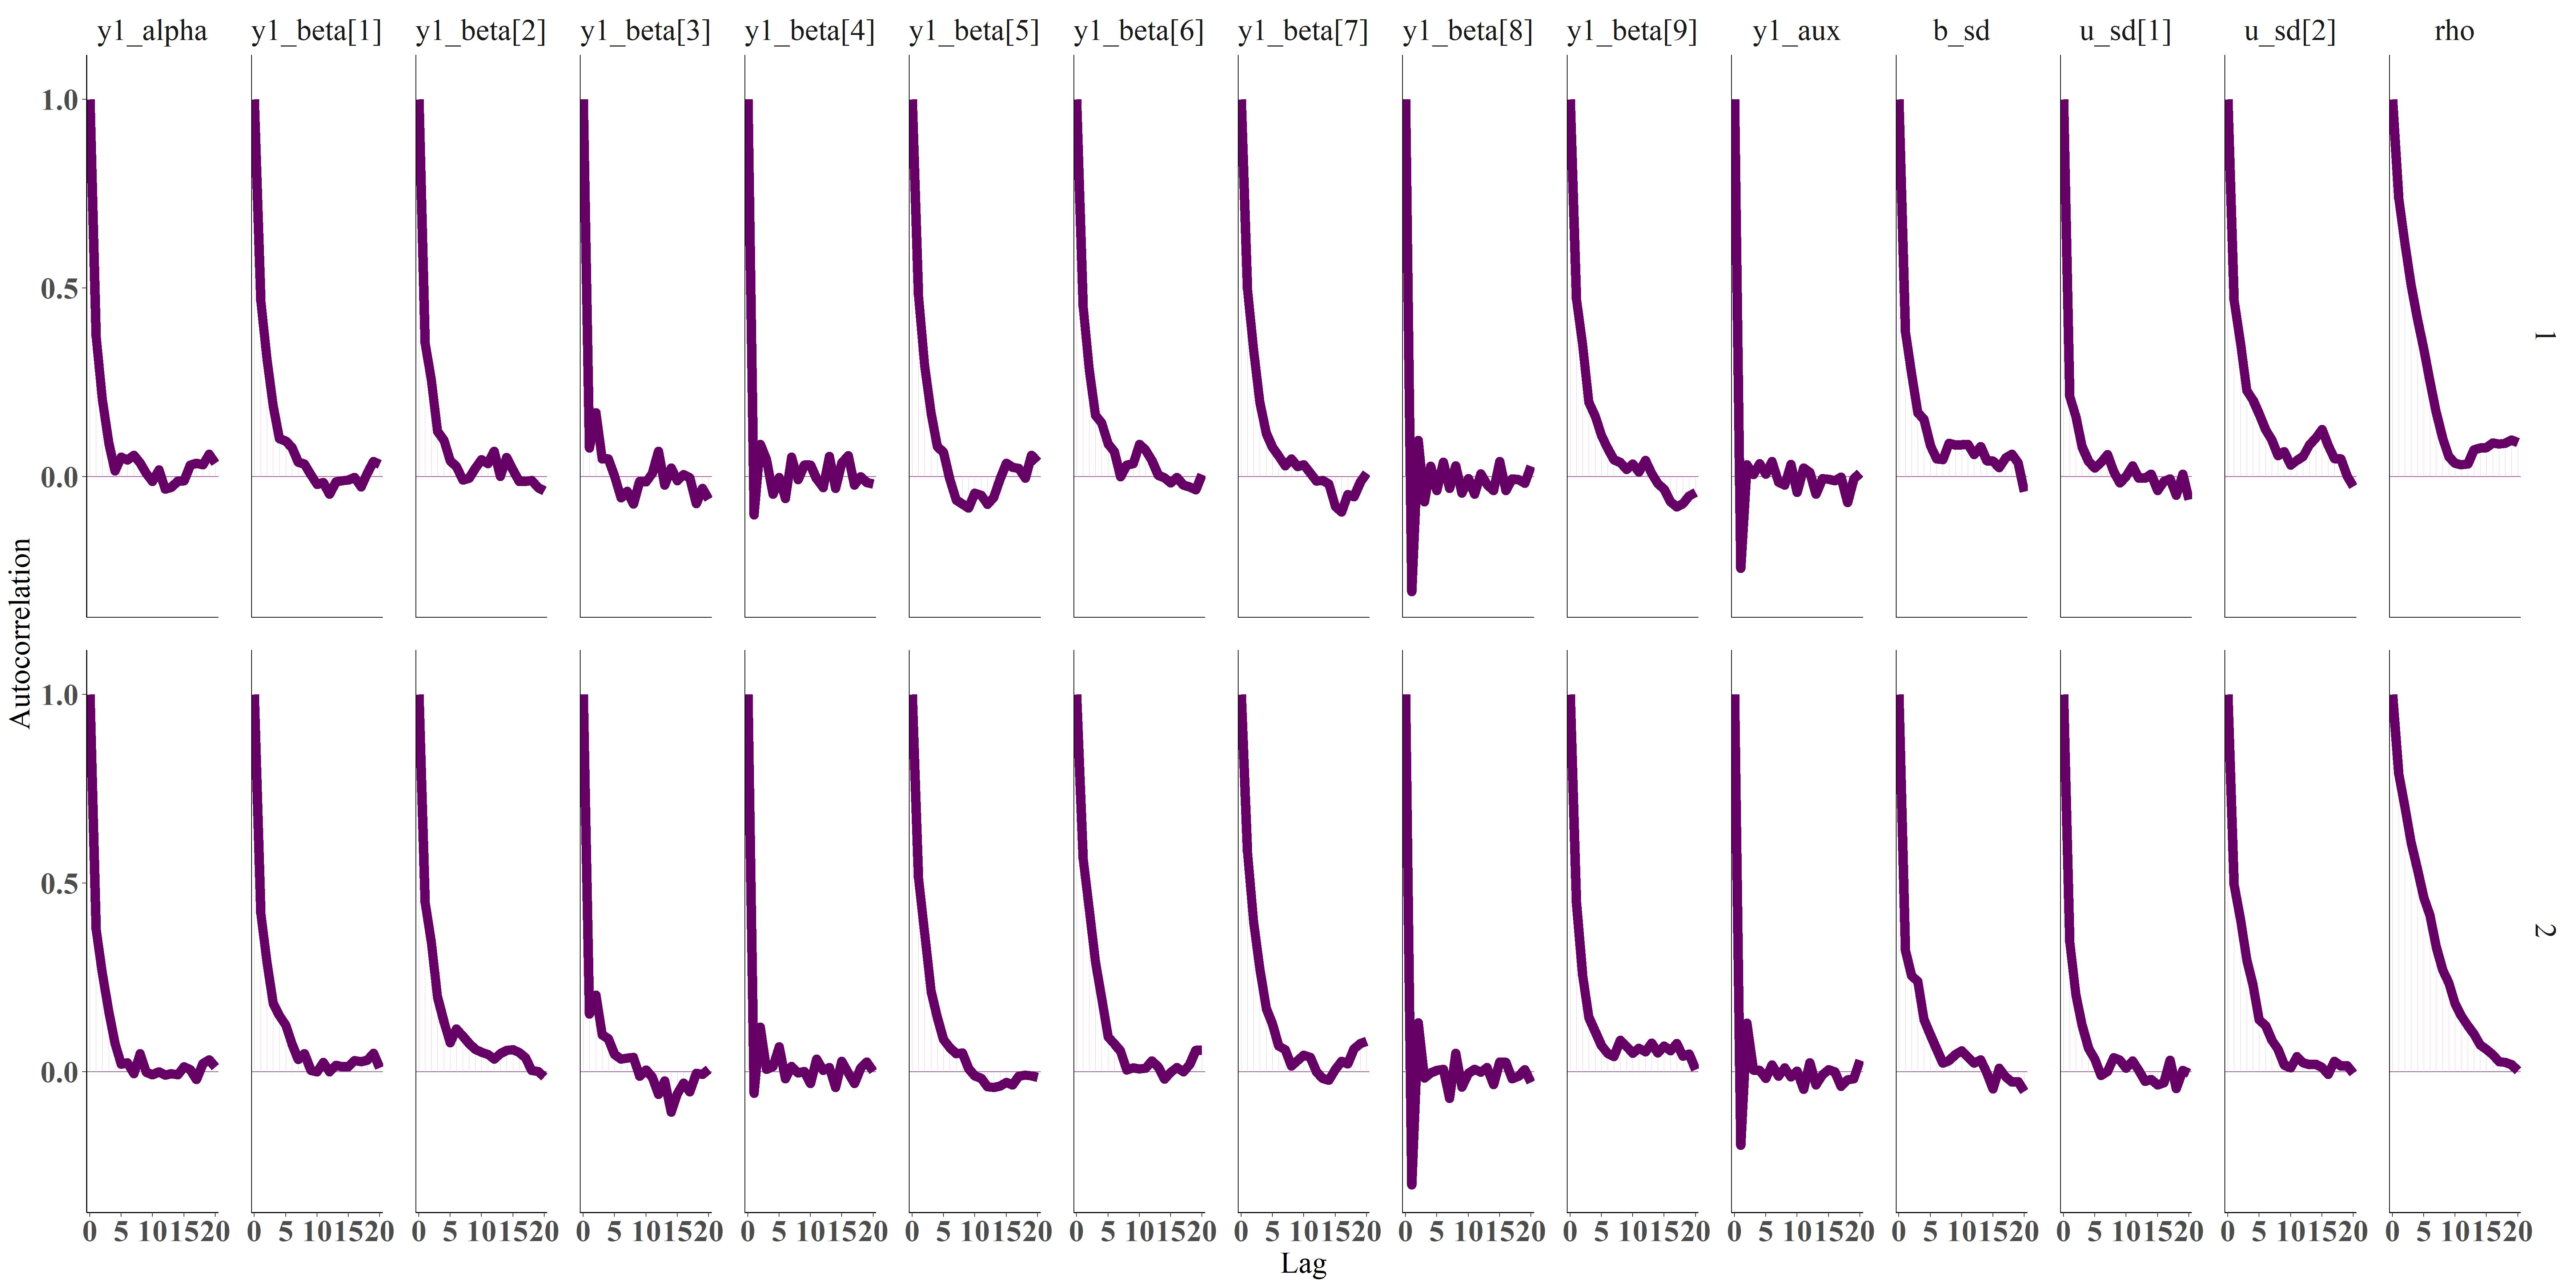
\includegraphics[width=\textwidth]{Figures/Chp3_acf_long.jpg}
\caption{Autocorrelation for parameters from longitudinal submodel}
\label{fig:acf_long}
\end{figure}

\begin{figure}[H] 
\centering
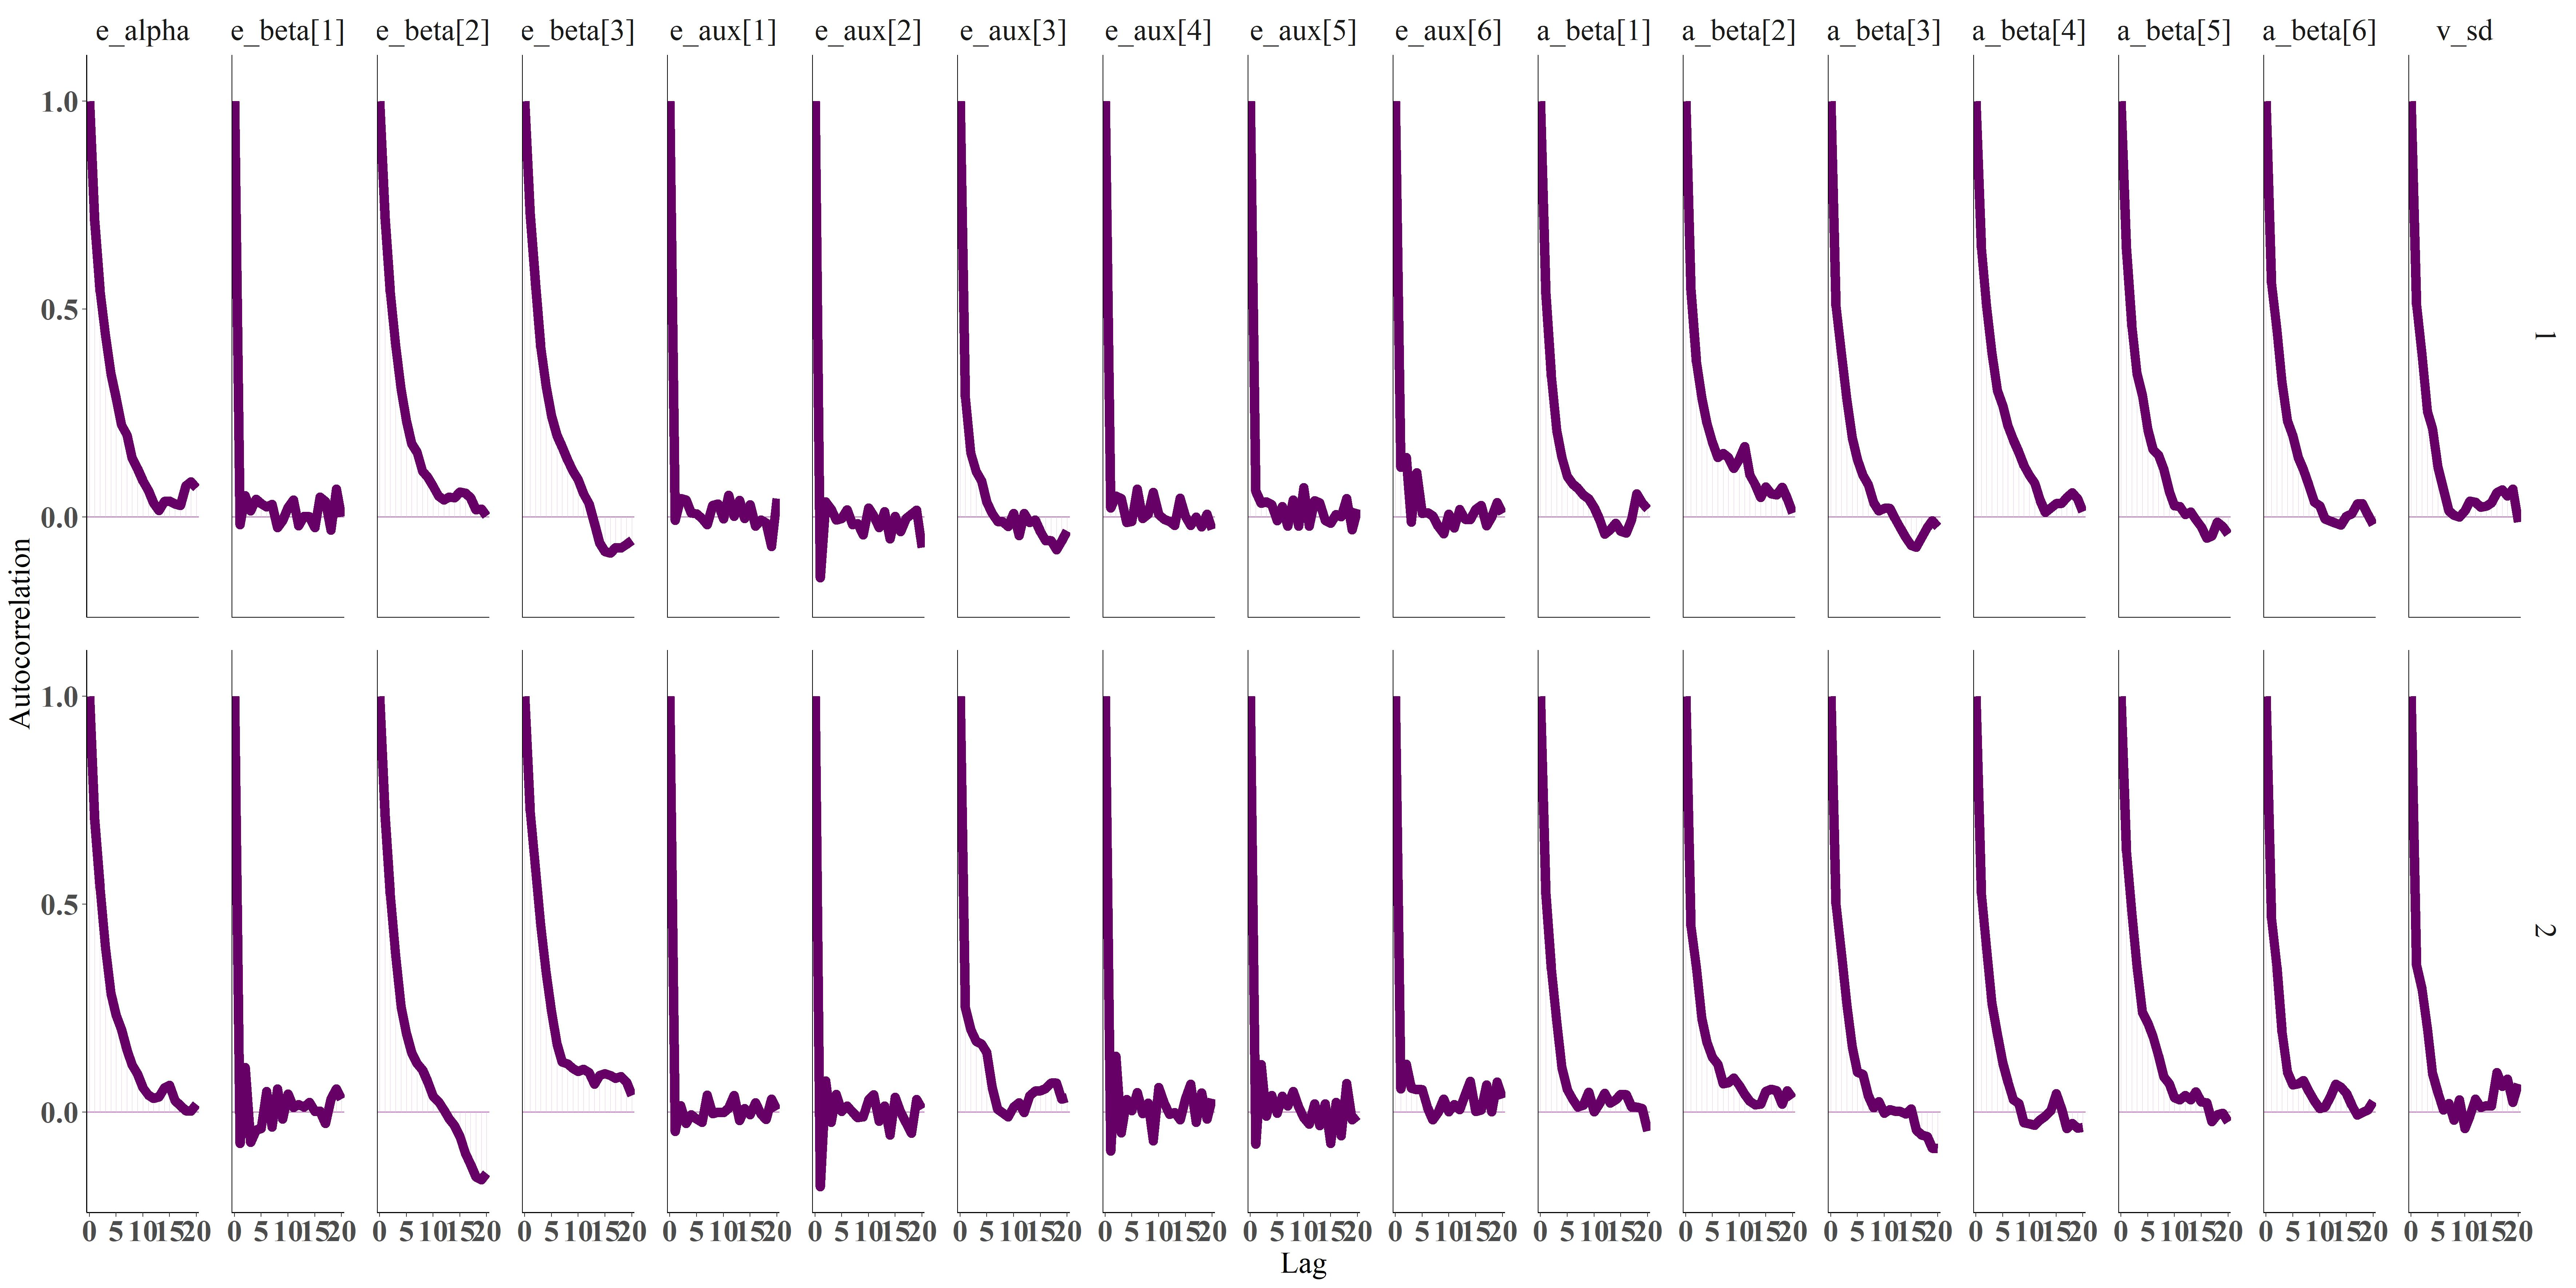
\includegraphics[width=\textwidth]{Figures/Chp3_acf_surv.jpg}
\caption{Autocorrelation for parameters from event submodel}
\label{fig:acf_surv}
\end{figure}


\begin{figure}[H] 
\centering
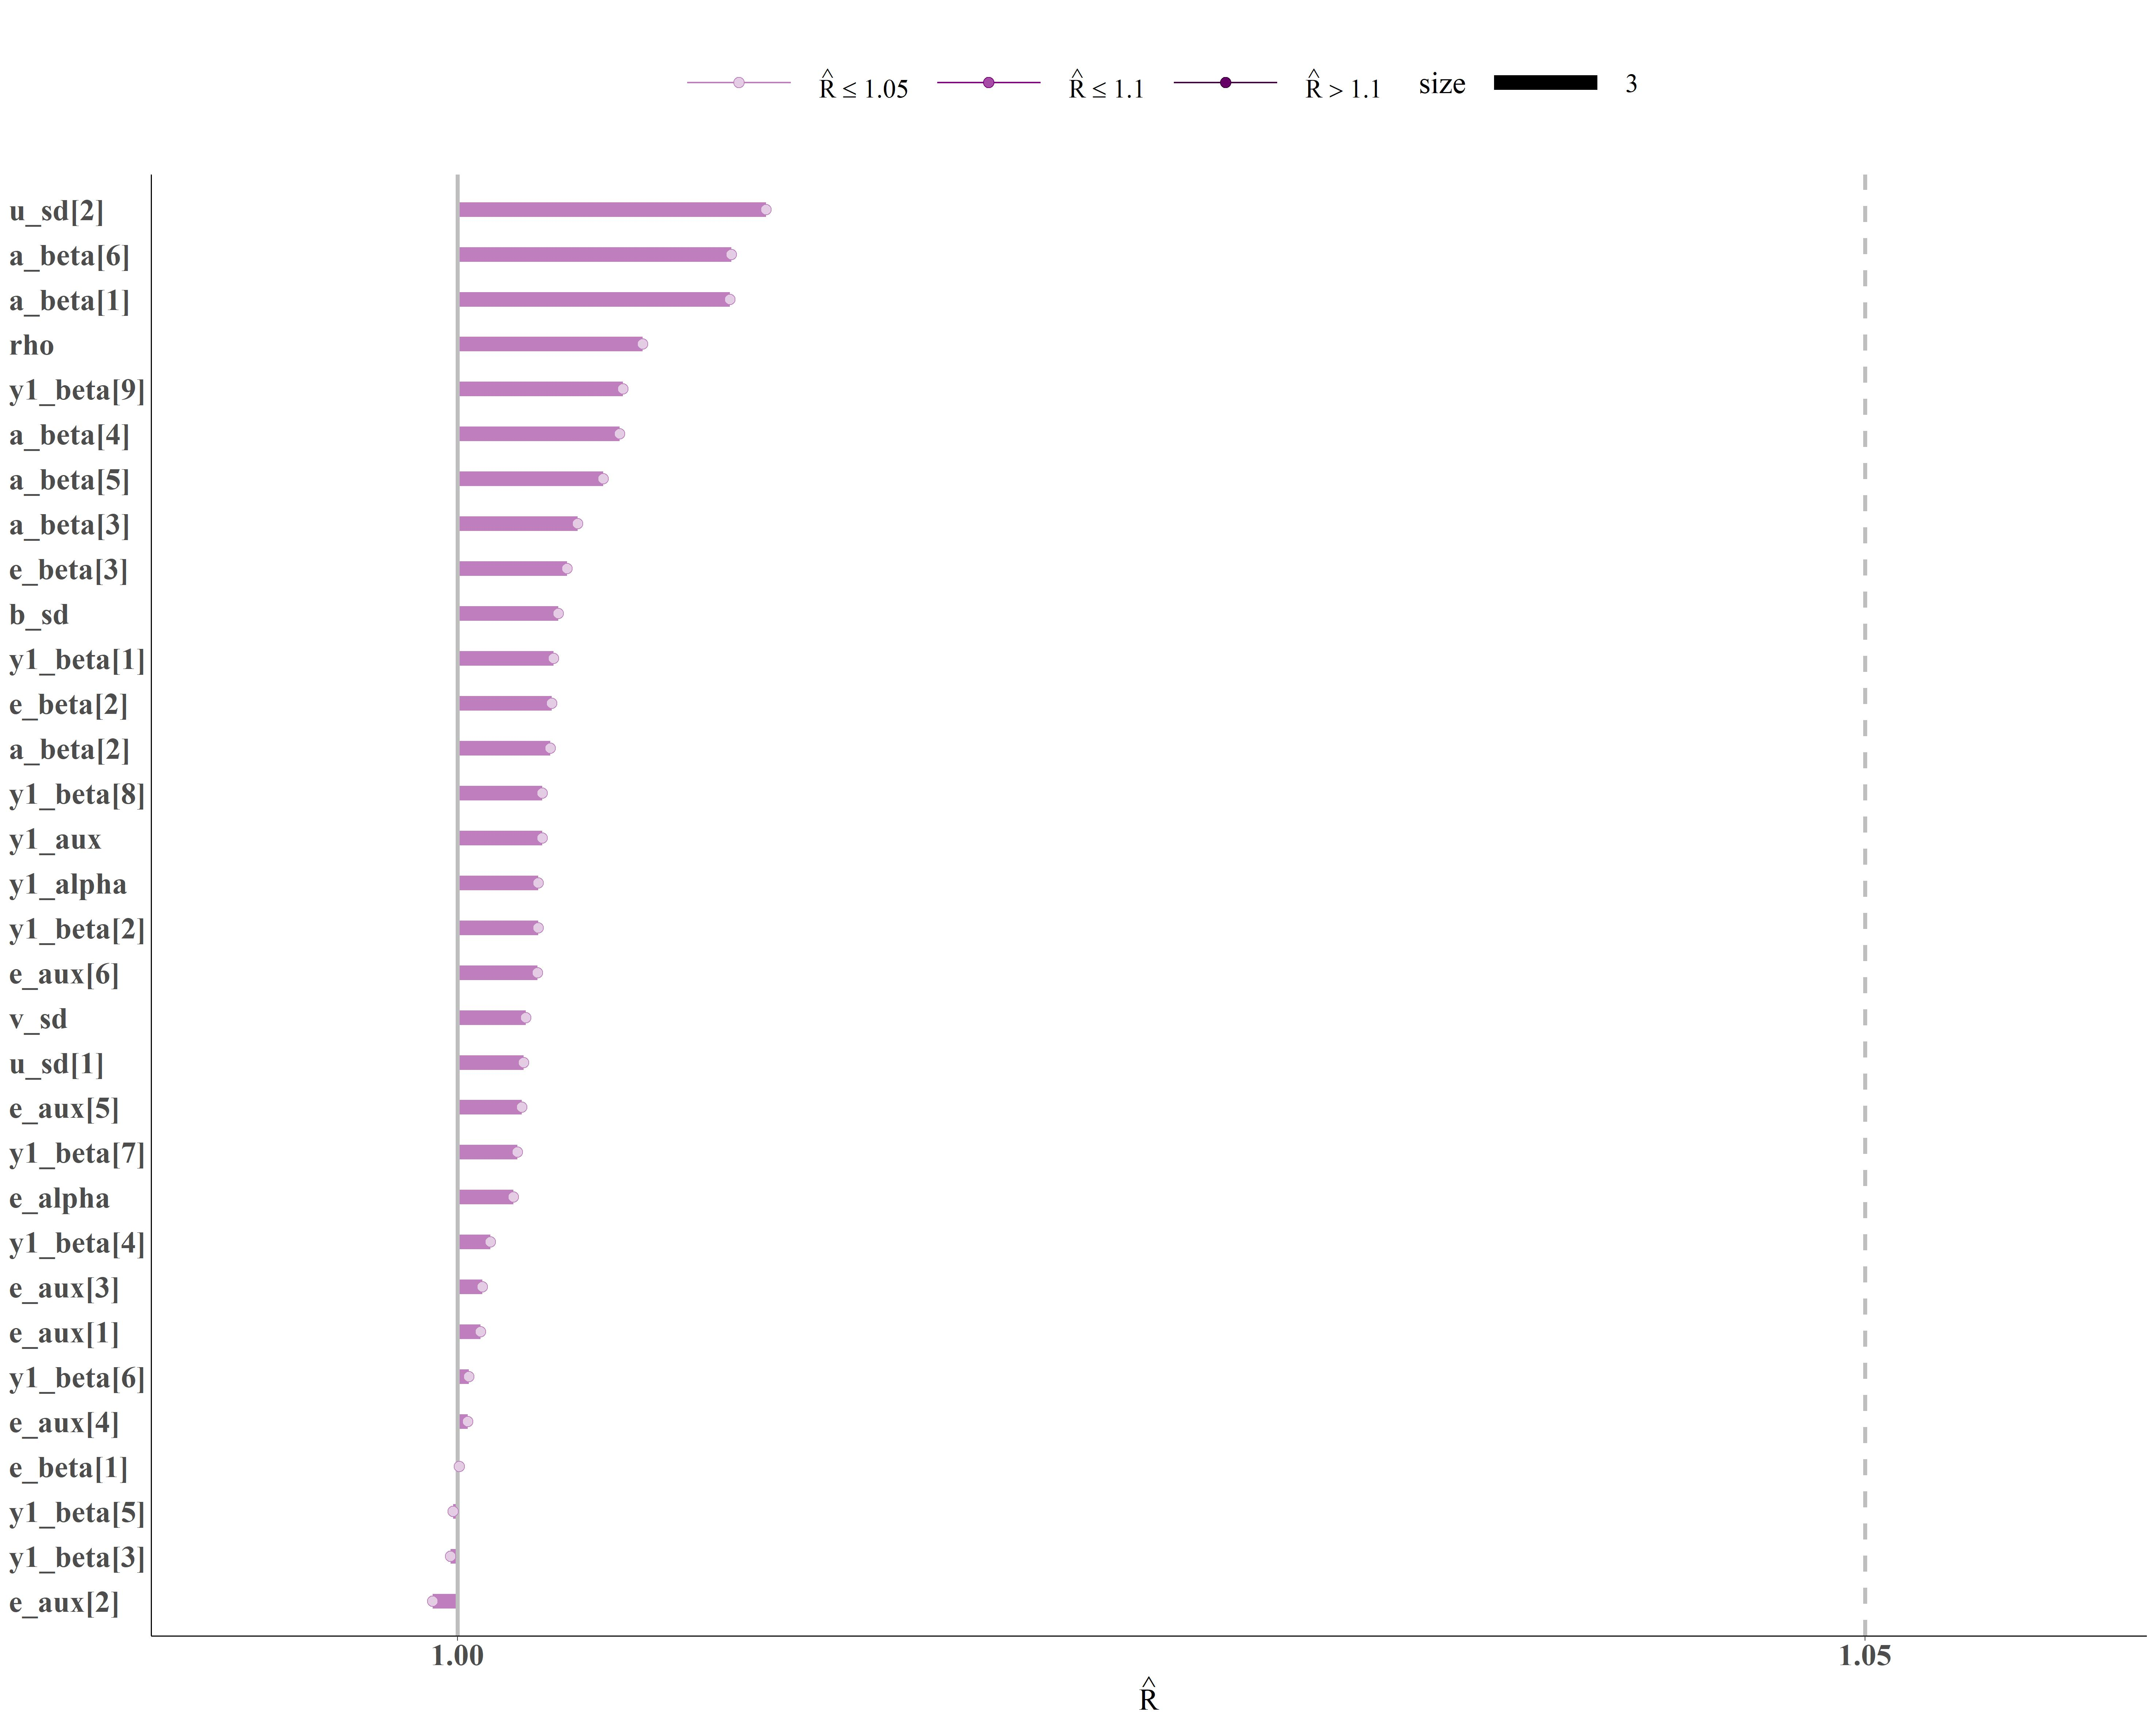
\includegraphics[width=\textwidth]{Figures/Chp3_rhat.jpg}
\caption{Rhat plot}
\label{fig:rhat}
\end{figure}


\section{Time and System}

Additional information about processing system and time are described in Table \ref{tab:system} and Table \ref{tab:time}. All models are estimated with 4000 iterations through two chains. The first 2000 draws are discarded as a warm-up sampling and the remaining 2000 are kept for the posterior inference for both simulated data and real data.

\begin{table}[H] 
\centering
\caption{Processing system}
\begin{tabular}{c|c|c}
\toprule
 & \bf Simulated data & \bf Real data\\
\hline
Platform & x86\_64-apple-darwin17.0 (64-bit) & x86\_64-w64-mingw32/x64 (64-bit)\\
\hline
Running under & macOS Big Sur 10.16 & Windows 10 x64 (build 19043)\\
\hline
R version & 4.0.5 (2021-03-31) & 4.0.2 (2020-06-22) \\
\hline
CmdStan & v2.28.2 & v2.29.1 \\
cmdstanr & v0.4.0 & v0.5.0\\ 
\bottomrule
\end{tabular}
\label{tab:system}
\end{table}


\begin{table}[H] 
  \small\sf\centering
    \caption{\bf Elapsed time in hours across scenarios}
 \begin{threeparttable}
\begin{tabular}{l|l|c|c}
\toprule
Association + Time scale & Model & Simulated data\tnote{a} (N\tnote{b} = 480) & Real data (N\tnote{c} = 440) \\ \hline
\multirow{2}{*}{Slope + Gap} & Joint Model &  0.18 & 9.16\\
                             & Two-stage Model & 0.05 & 2.86\\ \hline
\multirow{2}{*}{Slope + Calendar} & Joint Model & 0.26 & 3.82\\
                                  & Two-stage Model & 0.08 & 2.59 \\ \hline
\multirow{2}{*}{Value + Gap} & Joint Model & 0.18 & 8.17\\ 
                             & Two-stage Model & 0.04 & 5.31 \\ \hline
\multirow{2}{*}{Value + Calendar} & Joint Model & 0.15 & 7.10 \\              
                                           & Two-stage Model & 0.04 & 4.90\\
\bottomrule
\end{tabular}
 \begin{tablenotes}[para]
    \footnotesize
    \item[a] Averaged time per replicate; \item [b] Sample size (number of patients)
    \end{tablenotes}
 \end{threeparttable}
 \label{tab:time}
\end{table}


\section{Example Code}

We attach complete Stan program and partial R code for illustration purpose. For a complete version of R code and simulated data from Github use link: 


\subsection{Stan Program}
\begin{SingleSpace}
    \begin{minted}[breaklines]{R}

/***************************************************/
// Purpose: Fit proposed JM in the manuscript  
// Association structure: Slope/Value
// Risk interval: Gap/Calendar
// Assumption: i) full conditional independence; 
//             ii) LME: random intercept-slope; 
//             iii) Survival: extended stratified relative risk frailty model
// Author: Copyright (C) 2022 Grace C. Zhou
// Date: Mar., 2022
// Based upon:
// Copyright (C) 2015, 2016, 2017 Trustees of Columbia University
// Copyright (C) 2016, 2017 Sam Brilleman

/***************************************************/

functions {

  vector evaluate_eta(matrix X, array[] vector Z_u, int Dev_index,

                      array[] int U_id, array[] int C_id, real gamma,

                      vector beta, vector bVec, matrix uMat) {

    int N = rows(X); // num rows in design matrix

    int K = rows(beta); // num predictors

    //int p = size(Z_u);    // num group level params:intercept+slope

    vector[N] eta;

    if (K > 0) {

      eta = X * beta + gamma * Dev_index;

    } else {

      eta = rep_vector(0.0, N) + gamma * Dev_index;

    }

    //for (k in 1:p)

    for (n in 1 : N) {

      eta[n] = eta[n] + bVec[C_id[n]] * Dev_index

               + uMat[U_id[n], 1] * Z_u[1, n] + uMat[U_id[n], 2] * Z_u[2, n];

    }

    return eta;

  }

  
  /** 

  * Get the indices corresponding to the lower tri of a square matrix

  * @param dim The number of rows in the square matrix

  * @return A vector of indices

  */

  array[] int lower_tri_indices(int dim) {

    array[dim + choose(dim, 2)] int indices;

    int mark = 1;

    for (r in 1 : dim) {

      for (c in r : dim) {

        indices[mark] = (r - 1) * dim + c;

        mark = mark + 1;

      }

    }

    return indices;

  }

}

data {

  //----- Longitudinal submodels

  // population level dimensions

  int<lower=0> y_N; // num observations

  int<lower=0> y_K; // num predictors

  
  // population level data

  vector[y_N] y1; // response vectors

  matrix[y_N, y_K] y1_X; // fix effect design matrix

  vector[y_K] y1_Xbar; // predictor means


  // group level dimensions

  int<lower=0> b_N; // num center

  int<lower=0> b_K; // num center predictor

  int<lower=0> u_N; // num patients

  int<lower=0> u_K;// num patient predictor

  array[y_N] int<lower=0> y1_C_id; // center id 

  array[y_N] int<lower=0> y1_U_id; // patient id 

  array[u_K] vector[y_N] y1_Z; // random effect design matrix


  //----- Event submodel

  // data for calculating event submodel linear predictor in GK quadrature

  // NB these design matrices are evaluated AT the event time and

  // the (unstandardised) quadrature points

  int<lower=0> e_K; // num predictors 

  int<lower=0> a_K; // num assoc params

  int<lower=0> Npat; // num patients (equal to u_N)

  int<lower=0> Nevents; // num events (ie. not censored)

  int<lower=0> qnodes; // num nodes for GK quadrature

  int<lower=0> Nobs_times_qnodes; // Nobs x qnodes

  int<lower=0> nrow_e_Xq; // num rows predictor matrix

  matrix[nrow_e_Xq, e_K] e_Xq; // design matrix 

  vector[e_K] e_Xbar; // predictor means

  real norm_const; // norm constant

  int<lower=0> basehaz_df; // baseline hazard df

  vector[nrow_e_Xq] basehaz_X; // baseline hazard design matrix/vector (basis terms)

  vector[Nobs_times_qnodes] qwts; // GK quadrature weights with (b-a)/2 scaling

  matrix[nrow_e_Xq, y_K] y1_Xq; // fix effect design matrix at quadpoints

  array[u_K] vector[nrow_e_Xq] y1_Zq; // random effect design matrix at quadpoints

  array[nrow_e_Xq] int<lower=0> y1_Cq_id; // center id at quadpoints

  array[nrow_e_Xq] int<lower=0> y1_Uq_id; // patient id at quadpoints

  //----- Hyperparameters for prior distributions

  // scale prior

  vector<lower=0>[y_K] y1_prior_scale;

  vector<lower=0>[e_K] e_prior_scale;

  vector<lower=0>[a_K] a_prior_scale;

  real<lower=0> y_prior_scale_for_intercept;

  real<lower=0> e_prior_scale_for_intercept;

  real<lower=0> y_prior_scale_for_aux;

  vector<lower=0>[basehaz_df] e_prior_scale_for_aux;


  // lkj prior 
  
  real<lower=0> b_prior_scale;

  vector<lower=0>[u_K] u_prior_scale;

  vector<lower=0>[u_K] u_prior_df;

  real<lower=0> u_prior_regularization;

  int<lower=0> Dev_index;

}

transformed data {

  // indexing used to extract lower tri of RE covariance matrix

  array[u_K + choose(u_K, 2)] int u_cov_idx;

  if (u_K > 0) {

    u_cov_idx = lower_tri_indices(u_K);

  }

}

parameters {

 //----- Longitudinal submodel

  real y1_gamma; // intercept 

  vector[y_K] y1_z_beta; // unscaled coef

  real<lower=0> y1_aux_unscaled; // unscaled residual error 

  real<lower=0> b_sd; // center sd

  vector[b_N] z_b_vec; // unscaled center effect 

  matrix[u_K, u_N] z_u_mat; // unscaled patient effect  

  vector<lower=0>[u_K] u_sd; // patient sd  

  cholesky_factor_corr[u_K > 1 ? u_K : 0] u_cholesky; // cholesky factor 
 
 //----- Event submodel

  real e_gamma; // intercept in event submodel

  vector[e_K] e_z_beta; // unscaled log hazard ratio

  vector<lower=0>[basehaz_df] e_aux_unscaled; // unscaled baseline hazard coef

  vector[a_K] a_z_beta; // unscaled assoc params 

  real<lower=0> v_sd; // frailty sd

  vector[Npat] z_v_vec;// unscaled frailty effect

}

transformed parameters {

 //----- Longitudinal submodel
 
  vector[y_K] y1_beta; // scaled coef

  real<lower=0> y1_aux; // scaled residual error 

  matrix[u_N, u_K] u_mat; // patient effect  

  vector[b_N] b_vec; // scaled center effect 

  vector[y_N] y1_eta; // linear predictor 

 //----- Event submodel
 
  vector[nrow_e_Xq] y1_eta_q; // linear predictor at quadpoints

  vector[e_K] e_beta; // scaled coef (log hazard ratio)

  vector[a_K] a_beta; // scaled assoc params 

  vector<lower=0>[basehaz_df] e_aux; // scaled baseline hazard coef

  vector[Npat] v_vec; // scaled frailty effect
  
  //----- Longitudinal submodel 
  
  y1_beta = y1_z_beta .* y1_prior_scale;

  y1_aux = y1_aux_unscaled * y_prior_scale_for_aux;

  b_vec = b_sd * z_b_vec;

  if (u_K == 1) {

    u_mat = (u_sd[1] * z_u_mat)';

  } else if (u_K > 1) {

    u_mat = (diag_pre_multiply(u_sd, u_cholesky) * z_u_mat)';

  }

  //----- Event submodel

  e_beta = e_z_beta .* e_prior_scale;

  a_beta = a_z_beta .* a_prior_scale;

  e_aux = e_aux_unscaled .* e_prior_scale_for_aux;

  v_vec = v_sd * z_v_vec;

  //----- Longitudinal submodel 
  
  // linear predictor at observed time
   
  y1_eta = evaluate_eta(y1_X, y1_Z, 1, y1_U_id, y1_C_id, y1_gamma, y1_beta,

                        b_vec, u_mat);
                        
 //----- Event submodel 
 
 // linear biomarker predictor at event time and quadrature points  

  y1_eta_q = evaluate_eta(y1_Xq, y1_Zq, Dev_index, y1_Uq_id, y1_Cq_id,

                          y1_gamma, y1_beta, b_vec, u_mat);

}

model {

  //---- Longitudinal submodel

  // increment the target with the log-lik

  target += normal_lpdf(y1 | y1_eta, y1_aux);

 //---- Event submodel (Gauss-Kronrod quadrature)

  {

    vector[nrow_e_Xq] e_eta_q; // linear predictor at event time and quadrature points

    vector[nrow_e_Xq] log_basehaz; // log baseline hazard at event time and quadrature points

    vector[nrow_e_Xq] log_haz_q; // log hazard at event time and quadrature points

    vector[Nevents] log_haz_etimes; // log hazard at the event time only

    vector[Nobs_times_qnodes] log_haz_qtimes; // log hazard at the quadrature points only

    for (n in 1 : nrow_e_Xq) {
      
    // Step 1: event submodel add on contribution from association structure to
    // the linear predictor at event time and quadrature points
    
      e_eta_q[n] = e_Xq[n] * e_beta + y1_eta_q[n] * a_beta[y1_Cq_id[n]]

                   + v_vec[y1_Uq_id[n]];

      // Step 2: log baseline hazard (Weibull) at event time and quadrature points

      log_basehaz[n] = e_gamma + norm_const + log(e_aux[y1_Cq_id[n]])

                       + basehaz_X[n] * (e_aux[y1_Cq_id[n]] - 1);

    }

    // Step 3: log hazard at event time and quadrature points

    log_haz_q = log_basehaz + e_eta_q;

    // Step 4: log hazard at event times only

    log_haz_etimes = head(log_haz_q, Nevents);
    
    // Step 5: log hazard at quadrature points only

    log_haz_qtimes = tail(log_haz_q, Nobs_times_qnodes);

    // Step 6: increment the target with the log-lik

    target += sum(log_haz_etimes) - dot_product(qwts, exp(log_haz_qtimes));

  }

  //---- Log-priors

 //----- Longitudinal submodel

  target += normal_lpdf(y1_gamma | 0, y_prior_scale_for_intercept);

  target += normal_lpdf(y1_z_beta | 0, 1);

  target += normal_lpdf(y1_aux_unscaled | 0, 1);

  target += normal_lpdf(z_b_vec | 0, 1);

  target += normal_lpdf(b_sd | 0, b_prior_scale); // following Gelman 2008

  target += student_t_lpdf(u_sd | u_prior_df, 0, u_prior_scale);

  target += normal_lpdf(to_vector(z_u_mat) | 0, 1);

  // corr matrix

  if (u_K > 1) {

    target += lkj_corr_cholesky_lpdf(u_cholesky | u_prior_regularization);

  }

 //----- Event submodel
 
  target += normal_lpdf(e_gamma | 0, e_prior_scale_for_intercept);

  target += normal_lpdf(e_z_beta | 0, 1);

  target += normal_lpdf(a_z_beta | 0, 1);

  target += normal_lpdf(e_aux_unscaled | 0, 1);

  target += normal_lpdf(z_v_vec | 0, 1);

  target += normal_lpdf(v_sd | 0, 10);

}


generated quantities {

  real y1_alpha; // transformed intercept for long submodel

  vector[size(u_cov_idx)] u_cov; // var-cov for patient

  real rho; // correlation coef

  real e_alpha; // transformed intercept for event submodel
  
  //---- Long submodel

  y1_alpha = y1_gamma - dot_product(y1_Xbar, y1_beta);

  // Transform variance-covariance matrix for patient

  if (u_K == 1) {

    u_cov[1] = u_sd[1] * u_sd[1];

  } else {

    u_cov = to_vector(quad_form_diag(multiply_lower_tri_self_transpose(

                                     u_cholesky), u_sd))[u_cov_idx];

  }


  rho = u_cov[2] / (u_sd[1] * u_sd[2]);
  
   for (i in 1 : y_N) {

    log_lik_y[i] = normal_lpdf(y1[i] | y1_eta[i], y1_aux); // log-lik 

    y_tilde[i] = normal_rng(y1_eta[i], y1_aux); // posterior predictive dist

  }

 //---- Event submodel

  e_alpha = e_gamma + norm_const - dot_product(e_Xbar, e_beta);

}


\end{minted}

\subsection{R code}

    \begin{minted}[breaklines]{R}

library(cmdstanr)

file.jm <- file.path("JM.stan")
mod.jm <- cmdstan_model(file.jm)

fit.jm <- mod.jm$sample(
  data = standata.jm,
  chains = 2, 
  save_warmup = FALSE,
  parallel_chains = 2,
  refresh = 500,
  adapt_delta=0.95,
  max_treedepth=12,
  seed=202207,
  init = function() staninit.jm
)

\end{minted}

\end{SingleSpace}
